% Chapter 1

\chapter{Literature Review} % Main chapter title

\label{Chapter2} % For referencing the chapter elsewhere, use \ref{Chapter1} 

\lhead{Chapter 2. \emph{Literature Review}} % This is for the header on each page - perhaps a shortened title

%----------------------------------------------------------------------------------------

\section{Introduction}

In the past decade the world has been the epicentre of an extraordinary information explosion. This has been fuelled by the increased use of the internet coupled with the increased numbers of connected devices worldwide.  This rate of data growth has accelerated much faster than at any other point throughout history. This has affected not only machine generated data, but also enterprise application data - as both have continued to grow exponentially. This has posed industry experts with a great challenge - to develop new and innovative ways to evaluate and benchmark hardware and software technology and products. The studies have estimated that the total amount of enterprise data will only continue to grow \cite{gantz2012digital}. Data explosion not a singular incident. Its a global phenomenon that is growing every day. For example, with Asia now rapidly emerging as a major source of not only the data users, but also data generators. Similarly, with the increase of penetration in data driven computing, web and mobile technologies and enterprise computing, the new emerging markets have the potential to further add to this immense data growth \cite{kambatla2014trends}. 

The 21st century's global economic structure is transforming from an industrial economy into a new service economy. According to the results of a survey done by World Bank, the output of this service industry model takes up over 60\%  of the output in the world (sometimes exceeding 70\% in developed countries). This is partly because competition within the service industry is fierce, and this has become a huge focal point in the world's economic development. This means that service computing which provides re-usable architectures to support the modern service industry has come under the spotlight, and turned into an incredibly promising research area. Coupled with the increased popularity of cloud computing, more and more modern services are being deployed within cloud infrastructures in order to provide rich functionality. The number of services and users increasing every day, this has fuelled the explosion of data generation seen through services including mobile devices, social networks and large scale service oriented systems. It is because of factors such as these that the sheer amount of service generated data has become too large and complicated to be processed effectively by the more traditional approaches \cite{worldbank}.

It is no surprise, big data widely recognised and has attracted attention from the government, industry experts and academics. This is because big data is full of high volume, high velocity and variety information assets, and the increasing data requires new forms of processing to enable and inform enhanced decision making, insights, discoveries and further process optimisation. This issue was even mentioned by the Compliance, Governance and Oversight Council (or CGOC, which is an organisation focused on information governance) \cite{manyika2011big}. It is mentioned that, on average, information volume doubles every 18-24 months for most organisations, but the data creation speed is tremendous \cite{chen2014big}. In fact, its such a hot topic that in 2012 the Obama administration announced the big data research and development initiative, which explored how big data could be used to address the important problems facing modern governments \cite{wu2014data}.

The reaction to this phenomenon from leading IT companies such as SAGE, Oracle, IBM, Microsoft, SAP and HP has been staggering. These organisations have spent astonishingly on buying new software firms that specialise in data management and analytics. Data analytics industry on its own is worth over \$125 billion, and is growing at a rate of almost 10\% a year (this is twice as fast as the entire software industry). Because of this shift, effectively and efficiently creating values from big data has become an important research topic \cite{gantz2012digital}.

The emerging service oriented systems are not simple and often involve a huge number of services, each with complex services. The big data generated from these systems is typically heterogeneous, as well as being of multiple data and incredibly dynamic. And due to its nature, the increased system size and volume of data it contains, creating value from this became an incredible challenge. A few examples of the service generated big data being produced includes, trace logs, quality of service information and service invocation relationship. While similar to other kinds of big data, service generated big data initiatives span 4 unique dimensions \cite{ecoweb}:

\begin{itemize}
\item Amount: Modern large scale systems are full of every growing amounts of data which easily amasses terabytes and even petabytes of information.
\item Momentum: Certain time sensitive processes (such as bottleneck detection or quality of service predictions) could in fact be achieved as streamlined data streams directly into the system.
\item Variety: Both structured and unstructured data are generated in various data types, and this makes it possible to explore fresh new insights when analysing data in groups.
\item Collection: Detecting and correcting noisy and inconsistent data are important factors when constructing secure and trustworthy analysis. Establishing trust in big data presents a huge challenge, especially as the number and variety of sources continues to grow.
\end{itemize}

These four characteristics are unique to service generated data, and it provide the greatest challenge for data management and analysis. In order to achieve the full potential of this service generated through big data, developing exceptional technologies to effectively process large quantities of data within shorter processing times is a critical task. The transactional data or data sets utilised in this research is a kind of sub-set of big data phenomena, as the data sets are quite complex and the contributing sources are alike, the solution presented in chapter 3 could also be applied to any kind of data. 

\section{Acquisition and Data Analysis}

In the recent years getting data was a complicated and painstaking process and one that had to be done manually. For just a single voltage reading an engineer would need to go into the unit, manually attach a digital multimeter to the connections. The results would then need to be written down along with measurement values. The more complex the reading needed to get (for example a continuously varying signal voltage) the more difficult it is to read and measure accurately. Instead of just attaching the digital multimeter and taking reading, one would instead have to remove the original connection and instead connect to a separate standalone oscilloscope. And while it was possible to perform a visual inspection of the signal and perform a rudimentary analysis, it was challenging work. And not only was it a long and difficult task, it was made more difficult by the fact that each instrument was independent of the others and the limited available technology. However, the upside to this was that data management was a relatively easy task and our modern issues of volume and speed simply were not a problem \cite{mesurementsystems}.

There have been both major strides forward in technology and a significant decrease in the cost of hardware and software. Improvements such as the increase of microprocessor speed and storage capacity have helped form the catalyst for an explosion of data, one that is still increasing in size and speed every day. Now, the days of independent instruments are a thing of the distant past, with automated measurement taking over with hundreds of combinations of measurements and new devices that can function as a single cohesive system, instead of in multiple parts. It is because of these spectacular new developments that can make new discoveries and formulate new scenarios. Data acquisition rates have skyrocketed; peaking well within the mega-sample per second range every day, and technologies like high channel count systems are available to everyone. Data acquisition has become a profitable business in its own right and now there are even a range of affordable bench top data acquisition systems \cite{di2013data}.\\

In a nutshell, hardware concerns have been reduced along with primitive data collection tools. Recently, instead of focusing on the hardware vendors are now working to accelerate data collection even further, enabling engineers to break through previous data rates and resolution barriers. Worryingly, this has all happened so fast that it has inadvertently triggered a whole new wave of software issues to contend with. Instead of the previous hardware issues and the data, engineers are faced with unassailable mountains of data \cite{mininghighspeed}. The new technology provoked richer and faster data retention. The race has changed pace; now it is not about who can collect the data fastest, but who can make any sense of it \cite{chen2011essential}.

A growing number of modern technologies and complex products require data acquisition throughout nearly every stage from design and development to verification and testing. This means that engineers are facing the challenge of testing increasingly complex and delicate designs within smaller time-frames and ever shrinking budgets; all to meet the rising demand of customers who want high quality products for low prices. This means that quite a significant investment needs to be made in data collection to make the effort viable. There is hardware to consider, plus automation systems and the personnel need to perform tasks and analyse the data - which is still streaming in increasing volumes \cite{storager}.

Hand in hand with the huge volumes of data being collected comes the need to analyse it all and it is not something that has gone unnoticed by businesses. During the last decade business interest in data analysis has skyrocketed, and its not hard to see why. The competitive advantages a business can gain from analysing such data is huge which can provide decision makers with a solid grounding for decisions \cite{basicbusiness}. However, a business may want to implement sweeping changes based on the analysed data; the physical ability for change is limited by many other factors; such as staff knowledge, business supporting systems. This means that when a business depends on enterprise information systems, to modify or replace supporting information systems in order to make changes to business practice. Not to mention the most significant change modifying operational information systems is a must and these are often located within central repositories of automatic summarised data within huge data warehouses. That's why making changes based on data became a lot more complicated \cite{garcia2014using}. In the next sections, various web mining techniques will be analysed which will later be used in the system design and development process. 

\subsection{Web Mining}

Web mining is a technical term relating to the application of various data mining techniques to discover patterns and trends from the internet, and from a variety of enterprise data sets that are available to mashup applications. There are many different definitions of web mining, the definition found within the Gartner Group is the most comprehensive. Data mining is the process of discovering meaningful new correlations, patterns and trends by sifting through large amounts of data stored in repositories and by using pattern \cite{larose2014discovering}. Data mining is the process of uncovering hidden trends and patterns (that lend towards predictive modelling) and using a combination of explicit knowledge bases, sophisticated analytical skills and academic domain knowledge. This is also known as the process of producing new observations from pre-existing observations \cite{raju2014data}. This has also been described as the process of automatically extracting useful information and relationships from immense quantities of data. However if the purist approach is adapted, data mining does not involve looking for specific data; it simply finds patterns that are already present. This means that data mining cannot be used to unearth information in response to a question or hypothesis \cite{larose2014discovering}.

The continued increase in growth of online information combined with the unstructured nature of web data requires the development of powerful and efficient web data mining tools. Instead web mining tools are designed to dig out useful facts and knowledge from web pages, hyperlinks, page content and usage logs. It can be used in a number of ways to enable the streamlining of business process. For example, the web mining of an e-bank service can enable the employees of a bank to support e-business, helping to understand various marketing dynamics, new promotions or suggestions on the internet. Because of this there is now more of a tendency amongst banking companies and individuals to collect banks of information through web data mining, and to use that information for own interests to gain business intelligence, and this helps to make enlightened business decisions \cite{raju2014data}. Figure 2.1 shows various web mining types which are further discussed in the chapter.

\begin{figure}[H]
\centering
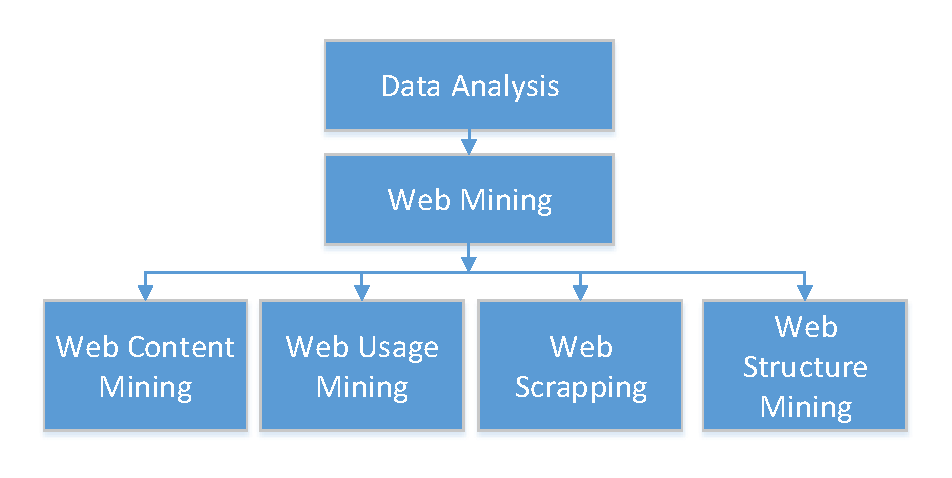
\includegraphics[scale=0.8]{chapter2/webmining_types}
\caption{Web Minning Overview}
\end{figure}

Web mining techniques are the result of an incredibly long process combining years of research. The web mining existed when the business data was first being stored on computers and on the internet, and evolution continued with drastic improvements in data access, and now the developments in real-time technologies that allow internet users to navigate through data quickly \cite{gargi2014dynamic}. Data that is gathered from surveys, manual input or from independently networked locations to define the data collection. Semantic Web has been developed to address current web problems, and it does this by methodically structuring the content of the internet and adding semantics before extracting the maximum benefits from the power of the internet. Sir Tim Berners-Lee defined the semantic web as an extension of the current web in which information is given well defined meaning, better enabling computers and people to work in co-operation \cite{berners2001semantic}. It is, in a word, a vision. The idea of having all of the data on the web systematically defined and linked together in a way that can be used and understood by machines. And not only for display purposes, but for automation, integration and the reuse of data across a whole liturgy of applications. Web mining also plays a pivotal role in achieving this, as it lets users quickly and easily find the information required.

Web based documents are split into three categories based on the structure: un-structured, semi-structured and fully-structured \cite{kim2015dynamic}. Structure data is usually in a normalised form such as databases \cite{park2014crowdfill}. Semi-structured data is not in a normalised form but contains markers or tags \cite{mansmann2014discovering}. Un-structured which doesn't have any pre-defined data model. There have been research studies into these categories, specifically on un-structured and fully-structured data, to look into the methods of  extracting semantics for ontology learning. In the research that focuses on fully-structured web documents benefits from a standardised syntax such as XML. However most of the web documents in existence today are in a semi-structured format, but only a few references are made to research that specialises in this format in extracting semantics for ontology learning. In most cases the plain text has been extracted from the semi-structured pages in pre-processing, therefore neglecting embedded information within the semi-structured format. Some other researchers focus on extracting semantics from more template driven web pages, and so these methodologies are limited both in usage and applicability \cite{liu2007web}.

\subsection{Web Usage Mining}

The term web usage mining was coined by Cooley \cite{mobasher2000automatic}, and is the application of various techniques used in data mining to discover and analyse the usage patterns of web data. It analyses user interactions with web servers including web logs or other database transactions from a group of related sites. However it has sparked privacy concerns and is currently the topic of much passionate debate. This is because the process includes mining data from the web server access logs, proxy server logs, browser logs, user profiles, registration data, user sessions or transactions, cookies, user queries, bookmark data, mouse clicks and scrolls and any other data as a result of interactions. Its aim is to discover the general patterns in web access logs, but in order to discover these patterns it is necessary to perform a few processes, including pre-processing, pattern discovery and pattern analysis \cite{wang2015design}. Web servers automatically record and store data about all of the user interactions whenever requests for resources are received. Analysing these web server logs, all kinds of different websites can better understand user behaviour and web structure, which in turn improves the overall design of this immeasurable collection of resources. Mining web usage pattern data, user can help in the progression of internet based studies; including those based on how internet browsers are used, and how the users interaction with the browser interface changed. These patterns can be put to use in gathering business intelligence, which will in turn improve customer attraction, retention and other aspects of customer behaviour \cite{claiborne2015self}.

\subsection{Web Scraping}

Web scraping is defined as the technique of automatic web data extraction, used in order to extract data from the core HTML of the website by parsing (the scouring and analysis) the web pages \cite{o2009web}. It does this by using programs specially coded for manipulation of web pages. Examples of this are: converting the web page into another format such as XML, or by embedding the browsers. It can be seen as fairly close to web indexing (this indexes web content using a soft-bot mainly adopted by search engines) but instead web scraping focuses on the transformation of completely unstructured web content into formally structured data, which can be stored and analysed in a central database. 

It can be used for a multitude of things, including online price comparison, weather data monitoring, web research, web content mashup and wed data integration. Not only that, but it can provide various levels of scrape like human copy and paste, text gripping (based on the UNIX command or regular expression matching facilities of programming languages like Perl), HTTP programming (HTTP requests to the remote web server), embedding web browsers, HTML parsers and web scraping software tools. A web server can be used to process to the scripting language, which in turn will produce the HTML response. Utilising text grabbing one can use the regular expression matching technique (where try to match a particular expression in the file) and find a match. Once a match has been found for the expression, users can then pick the values before or after it. The main limitation of scraping programs which are required to update frequently, which can increase the maintenance costs \cite{munzert2015automated}.

\subsection{Web Structure Mining}

Web structure mining is a field of research entirely focused on identifying more preferable documents by using the analysis of the web link structure \cite{kosala2000web}. The idea is simple: a hyperlink from document A to document B implies that the author of document A thinks that document B contains worthwhile and useful information. Web structure mining seeks out and exploits the additional information that can be found within the structure of the hypertext. Because of this one of the most important application in this area is the identification of the relevance of these linked pages which appear equally important when analysed, especially when one look at the content in isolation. To illustrate: a hyperlink induced topic search analyses the hyperlinks topology by discovering authoritative information sources for broader search topics. To find this information, it goes to authority pages, which are defined in relation to hubs as the counterparts. Hubs are otherwise known as pages that link to multiple related information authorities. For example, Google owes its massive success to its page ranking algorithm, which states that the relevance of any page increases with the number of outbound links (hyperlinks to it from other pages); more so if those other pages are relevant \cite{renu2014implementation}.

\subsection{Web Content Mining}

This is an automatic process of the internet which extracts patterns from web contents, data and documents (such as HTML files, images or emails). This already goes beyond simple keyword or key phrase extraction; instead it can take full advantage of the semi-structured nature of the web page text, and can use it to detect co-occurrences of terms within the texts. For example, user can also discover  trends over time, which could indicate a surge or decline of interest in certain topics (such as the programming language Java) \cite{mobasher2000integrating}. Another area this can be applied in is event detection; using web content mining in the identification of stories in multiple continuous news streams that correspond to new or previously unidentified events \cite{yadav2015web}. 

\section{Data Representation}

Visualisation has been a prominent and fast moving field for a long time, as a sub-field within science, statistics and graphs, it has only been recognised as its own entity since the mid to late 80s \cite{wilkinson2009history}. In this field, the full depth of the seminal work conducted, the strength of visualisation is drawn from its background; years of statistics and graphic design that form the basis for something much stronger. The process known as information visualisation is done by converting data into a series of interactive interfaces to allow users to understand data problems, unearth hidden patterns and explore the data with a more intuitive and analytical approach. Traditionally, visualisation uses aggregate data and transforms this into visual images, to allow users to see the big picture at a single glance \cite{chen1999information}.

Information visualisation is a process, also known as a visual medium between data and the people trying to understand it. It also works as a bridge to establish interactivity between source and operator for analysis and decision making purposes. The ultimate goal of information visualisation tools are to provide and improve data perception, correlation, interpretation and exploration. Setting apart good and bad practices in information visualisation can sometimes be difficult to define the parameters in order to establish quality visualisation. These are key visualisation attributes \cite{carr1999guidelines}:

\begin{itemize}
\item To analyse or examine entire data set.
\item Ability to see non-aggregated elements of subsets.
\item Customisation and filtering to analyse data at multiple degrees.
\item Making additional information available to an action which is performed by the user.
\item The ability to relate data items with similar characteristics to form and build relationships.
\item The ability to undo an action made and show the steps performed up to the current point. 
\end{itemize}

In order to analyse data problems in depth, a number of different techniques have been invented to explore data \cite{wang2000guidelines, north2000snap,pillat2006coordinating,eick1999visualizing,stolte2002polaris}, allowing users to dig deeper and find trends and patterns. For example, both Tableaus visual spreadsheet \cite{tableau} and SpotFires visual data exploration interface \cite{spotfire} are utilised by business managers for routine data analysis. The existing visualisations tools such as pixel-oriented visualisation \cite{keim2002pixel}, where large transactional data sections are represented by each pixel in the visualisation, digging into data to explore patterns and trends. For example, in the VisDB system \cite{keim1994visdb} each individual pixel is arranged and coloured to indicate the items relevance to a user query. Equally well known technique that uses pixel-level visualisations the Seesoft software visualisation technique. This technique maps each line of source code and connects them to a line of pixels. These techniques have been used in a wide variety of ways including to build interactive decision tree classifiers, which would be based on the visualisation of training data \cite{eick1992seesoft}. Another approach to non-aggregated data visualisation is known as value cell visualisation \cite{keim2007value}, and this is usually displayed in bar chart format. Pixel orientated visualisations became a necessity within data visualisation in part because all other visualisation practice (such as pie charts, bar charts, x-y plots) are a form solely focused on the aggregation of data, which in  turn restricts the number of data values able to be visualised. While this is a working model, this dilutes our understanding of the data and the visualisations do not always give the precise and accurate information to the decision makers. The pixel bar charts and value cell bar chat visualisations were a fantastically successful way to visualise non-aggregated data, but this left a lot to be done in terms of multi-coordinate data visualisation and data relation in visualised form - with a lot of gaps still in the process. Using multiple view systems, can use two of more distinct views to support the investigation process of a single entity. However a view is only considered distinct when compared to other views if it allows the user to learn the different aspects of the conceptual entity - whether by presenting different data or by emphasising different aspects within the same data  \cite{keim2002pixel}.

The Snap-Together \cite{north2000snap} is a data analysis and information visualisation system that supports the use of several different types of data set. The coordination of this data is limited to the selection of data items the DEVise can represent, and multi-dimension data is separated by the DEVise into several multi-dimension visual representations. Users can then move on to view integration, which is accomplished by zooming in and using multi-coordinate views on the data to explore it further.  This view supports a coordinated series of data items, and is recognisable by a selection, highlight and colour mapping dynamic queries of the data. Approaches such as this multi-coordinate visualisation provide a solid understanding of data, and helps in the data validation and cross examination of data to find hidden patterns and trends, as well as providing critical information to the decision making process. However, when trying to see the original data even these multi-coordinate practice fall short of the mark. In order to resolve this, the proposed linked data visualisation which provides a link and relationship between different data aspects \cite{abraham2014multi}.

It is often said; a pictures worth a thousand words. But does such an intelligent analytic speed imply that people can absorb visual information in a more efficient way than information conveyed through words? Can we happily say, for example, that people learn and remember visually presented information better than they remember verbal information? There have actually been a number of experiments that have tried to demonstrate this very fact, with mixed results. Some authors find no significant link between presentation style (visual vs verbal) and recall rates unless individual preferences are taken into account \cite{butler1996multimedia}, on the other hand visual business intelligence is on the rise, analytical tools are becoming mainstream \cite{basole2014visual}. However, according to studies visual intelligence is the most dominant type of intelligence, and many researchers and teachers surveyed \cite{survey1} believe that most of the students learn best through a visual medium.

\begin{itemize}
\item  approximately 65 percent of the population are visual learners; 
\item the brain processes visual information 60,000 faster than text; 
\item 90 percent of information that comes to the brain is visual”. 
\end{itemize}

Why does it appear that we understand words/numbers and graphs differently? People interpret numbers and graphs differently because these are processed differently in the brain. Numbers and words are generally handled by the verbal linguistic system and graphs are handled by both the non-verbal linguistic system and the limbic system. The bit rate of the visual system is about 10 million bits per second \cite{koch2006much} and the rate of reading is approximately 150-400 words per minute. To understand how this works, and provide a foundation for further reading, a very brief review of the relevant neuroscience seems in order. Following are some neuroanatomical details of the human brain. However, there are many other important aspects of cognition such as perception, memory, emotional modulation.

In the digital age, and there are huge volumes of data and information available within organisations, which if handled incorrectly can lead to data paralysis. To avoid this, it is increasingly important for organisations to ensure they are using the information effectively and that includes using data visualisation to explore and present the information. Information visualisation is the perfect way to present data graphically and take advantage of the visual nature of people allowing users to amplify cognition and gain better results. Through visual stimulus. The information visualisation used within the Spotfire \cite{koch2006much} and IBM Cognos software \cite{ibmcognos} provide visualisation techniques such as histograms, bar graphs, scatter plots and tree maps. These visualisation techniques are used in computerised environments in order to amplify human cognition in 5 key ways:
\begin{itemize}
\item  Increasing the memory and processing resources  available to users;
\item  Reducing the search for information;   
\item  Enhancing the detection of patterns;   Enabling perceptual inference operations; 
\item  Using perceptual mechanisms for monitoring  systems;   
\item  Encoding information in a medium that enables  easy manipulation.  
\end{itemize}

As discussed above, the information visualisation science is such an important contribution in learning fast, the same principle could be applied with learning from complex data. The next section of this chapter will discuss various types of visualisation which will be introduced in the research model for greater understanding of data problem.

\subsection{Bar Charts}

In terms of presentation graphics, bar charts are certainly the most simple and effective method, however it can only show aggregated values such as total sales for each months, making it limiting. Because of this, valuable information often gets lost in translation and is difficult to analyse. In fact, the usefulness of bar charts is especially limited if the user is interested in exploring the relationships between the different attributes available such as product price, number of orders and quantities.  The reason for this limitation is that multiple bar charts for different attributes do not support the discovery and exploration of interesting subsets which is one of the most important elements of data mining. A number of visualisation techniques have shown that the usefulness of data exploration in the discovery of patterns and trends is key in multi-dimension data. For example, both Tableaus visual spreadsheet \cite{tableau} and SpotFires visual data exploration tools \cite{spotfire} are widely used by business managers to aid in daily decisions making. Space filling techniques such as squarified treemaps and screen-filling curves are also used to help visualise hundreds of data records daily. For the aid of visualising even larger amounts of data, pixel-oriented techniques (which, as explained above, use each pixel to represent one data value) can be used for effective understanding. In the VisDB system \cite{keim1994visdb} for example, each pixel is arranged and coloured to indicate an items relevance to a user query. However, bar charts used with a combination of other simple charts exploration data could help in addressing data problems.

\subsection{Multi-coordinate Visualisation}

Multi-coordinate view is a very specific term for the exploratory visualisation technique that enables users to explore the data in full. The overall idea for the technology and premise for the technique is that it helps users to understand data better in a presented form displayed in various representations to allow an overall image. On the one hand, users want to view complex and intricate data in a simple way of exploring and deciphering, discovering facts and patterns that aren't easy to find. These complex data investigations require the user to consider many different scenarios in order to compare the visualisations generated from multiple data sets. To aggregate and mine such vast arrays of data, sometimes fusing data from many diverse data sets and create new information and insights, while still maintaining the ability to roll back to the previous incarnation, can be a difficult task. This is especially true when experts are looking at the same sets of data, but comparing and discussing different exploration paths and conclusions. Such complex and delicate analytic investigations require the right exploratory tools, allowing for a comprehensive analysis with intuitive functions \cite{roberts2007state}. 
On the other hand, some users might already be too familiar with the techniques these programs use, and because the applications on autopilot, missing out on some of the riches of the underlying data. Utilising a visualisation design environment which allows users to examine the different representations of the data while managing the interactions and automatically coordinating operations between the different views. Using this approach to open up new and insightful facts and relationship information about the users data without sacrificing accessibility.

In a nutshell, the purpose of a good visualisation application is to allow all users to have an interactive dialogue with the data. It can be quite challenging and time consuming to find, collect and make sense of large volumes of data, and how application makes the process of handling such data, even if it is from multiple sources of various types, much easier for the end user. The user's goal in this situation is simple to understand the data, view trends, find unusual patterns and organise this information in any way that is desired. Allowing unrestricted access to the data and its deeper meanings, and are able to discover and compare differences and similarities in the data sets, examine the outcomes of various scenarios and develop grounded theories through systematic analysis. In order to achieve greater insights to data problems, the visualisation systems should provide interactive visualisation experience. Which enables users to dig deeper and discover new meaning in the data. These interactive systems are the heart of the coordinated multiple views technique, therefore allowing insights through data analysis \cite{zhang2014visual}.

\subsection{Multi-dimension Data Visualisation}

The development of the modern database system, users can now find multi-dimension data is a prominent presence in a wide variety of fields. This is largely because individual people on own lack the time and skills to find multi-dimension data, limiting the knowledge and ability to visualise multi-dimension data to help in decisions. Creating an easy to use and highly interactive visualisation model that allows users to dig for knowledge within the data has become the main challenge within the visualisation field. The unique technology used within multi-dimension data visualisation is adopted primarily from the data mining area of visualisation. Such techniques are used as a communication tool, to help us generate the initial view, resolve complex structure issues and display the data and analytical results in order to give us a clearer perspective. However this is quickly changing \cite{mothe2003doccube}. The general scope for visualisation is a much more comprehensive collection of information, with many different techniques. In multi-dimension data visualisation, system has a number of display options which are viewed as the traditional paths - such as parallel coordinates, word shape or scattered matrix. These methods work perfectly for smaller amounts of data, but when to start moving into larger volumes these methods start to fail. The answer to this problem lies with multi-dimension data coordinates,visualising data in more than one dimension for trends and patterns exploration \cite{khandelwal2014multi}.

\subsection{Multi-attribute Visualisation}

The geo-spatial data sets, while often unstructured in nature, typically have size, distances, directions, locations and altitudes, giving an inherent positional structure and shape. But maintaining the boundaries of such spatial objects imposes major structural and positional constraints on our choice of visualisation techniques. The data associated with such spatial objects can often be multiple variate, making visualising such multiple variate spatial objects a very challenging task \cite{shneiderman1996eyes}. In particular, time varying geo-spatial data volumes are often so large that interactions among these become too complex, and it is often difficult for users to understand how the data changes over time when the individual images are viewed in isolation, so in order to show both spatial and temporal data changes over periods of time, special visual methods are needed to unearth the important patterns and relationships within the data \cite{maceachren2005visualizing}. These changes in the spatio-temporal data might be existential (such as appearance or characteristics) or it may be spatial (changes in shape or position) or even attribute changes ( such as changes in non-spatial characteristics of spatial objects). In this explanation, to deal with attribute changes within spatio-temporal data. Using more trajectory based techniques like those proposed \cite{skupin2000metaphor}. Users are able to represent changes in attribute as the movement of objects across a two dimension self organising map surface. The computational changes are made to complex data in order to distort the spatial locations, patterns are often more visible. In stark contrast, our application required these spatial location points to be preserved, not altered. Solcum \cite{slocum2001cognitive} suggests that spatio-temporal data that is associated with point locations can be displayed using animation, small multiples or changing maps, as evidences in the tool MapTime. However,  Andrienko mentions that animation is often not an effective method for analysing the change in attribute values, due to the effects of change blindness \cite{andrienko2003exploratory}. Skupin \cite{slocum2001cognitive} argue that the need for temporal visualisation methods for census data cannot be fulfilled simply by using multiple maps placed side by side, or by using percentage change maps. This is owing to the large size of census data, and it is imperative that the task of identifying change for visual detection is not left to simple human users. CommonGIS \cite{andrienko2002testing} offers multiple techniques for visualisation, where a coherent display of multiple maps is used to compare several different scenarios. In addition, CommonGIS also provides choropleth maps, time maps and time aggregates to visualise spatio-temporal data more effectively. However, with the execution of choropleth maps, most of the techniques provided in CommonGIS represent data by using graphs, time series charts, histograms and scatter plots. Instead our application aims to visualise information on the map while still maintaining the spatial boundaries of the planning polygons, since these are what help the user understand the data more effectively \cite{tahir2014geovisual}.

\subsection{Business Analytics Through Visualisation}

There are many definitions for the term analytics, with professionals in different fields viewing it in very different ways. However the common ground that may find, is that analytics is the processes of reviewing a set of insights generated from accurate historical data, and developing a series of actionable decisions of recommendations based on it \cite{melpignano2012platform}. Recently there has been a development from The Institute for Operations Research and Management Science (otherwise known as INFORMS) that has created a major initiative for the organisation and promotion of analytics. By the definition INFORMS present, analytics represents the combination of computer technology, management science techniques and statistics to help solve real problems. This has sparked many other organisations to develop the interpretations and motivations for the use of analytics \cite{keim2008visual}.

The descriptive analytics (also known as reporting analytics) refers to a detailed knowledge of activity within the organisation, and further to that the identification and understanding of the underlying trends and causes of the activity. To do this, there is a certain amount of data source consolidation and availability required to gather all the relevant data to analyse and ensuring that this is all in a form that enables reporting and analysis. This creates a data infrastructure, and user can use this to develop the required reports, queries, alerts and trends using the various reporting tools and techniques. This process and the technology used within it has become a key component in how user visualise and deal with data. Using the latest available tools in visualisation user can move on to developing accurate and powerful insights into the inner operations of our organisation \cite{haas2011data}. 

The predictive analytics is a process that sets out to determine what is likely to happen in the future based on trends. This form of analysis uses statistics as a firm basis, as well as newer techniques that have been more recently developed in the field of data mining. The goal of using these techniques in data analysis is to be able to predict the behaviours of customers likely to switch to a competitor company, how much of what they will buy next and what special offers or promotions would evoke responses. In developing these predictive analytical applications a number of techniques were used, including various classification algorithms. These included decision tree models and neural networks (similar to those used to predict box office success) and clustering algorithms (to segment customers for targeted promotions). Combining these with well known association mining techniques user can create estimations of the relationships between purchasing behaviours (what a customer is likely to purchase based on previous purchases). These analytics are essential to retailers in the process of promoting or recommending products for the customers \cite{shmueli2011predictive}. 

The third and final category of data analytics is known as prescriptive analytics - the aim of which is to examine both the current trends and the predictions made via predictive analytics, and use the information to make educated decisions. As a group these techniques are often referred to as operation research or management science, and are used to optimise the performance of any given system. The overall aim of this technology is to provide recommendations or provide a concrete decision for a specific action. Recommendations from this model can come in the form of yes/no decisions, defined amounts (if this was the aim, e.g. the price for a specific item) or even a complete set of production plans based on reports. The decisions created can be presented in either a decision making report, or used directly in an automated decision rules system (e.g. airline pricing systems). Because of this versatility, prescriptive analytics can also be known as Decision or even Normative analytics \cite{davenport2007competing}. 

There are hundreds of different ways one can measure and evaluate the success of a business. To use profit margins, staff performance rates or sales figures. But the most important way to do this is through simple client satisfaction. In some cases businesses will view this as more important than the business profit. However determining levels of client satisfaction is not as easy as it sounds and is instead determined by a specific sequence of information and decisions about the quality of services, offered products and getting to know the clients among others. This can be determined by predicting the needed improvement of infrastructure based on a client growth rate, defining the need for expansion with variety of specialised products, or by establishing detailed profiles of the clients, including which of the products or services are required, and when. The bigger question here has yet to be asked if the criteria are known and established, then why are so many businesses having trouble achieving the goals? Well, this could be something as simple as the fact that analysing such enormous amounts of data is by no means a trivial task and that the system reports generated from that data don't always hold the answers. It is because of this variable that the decision makers in charge often don't have enough information to complete the picture - or in some cases have gleaned incorrect information because the correct data is lost in an endless and overly complex report. Because time is such a critical factor in business decisions, being presented with a set of static data is also not the answer - as this can skew the picture \cite{bertsimas2014introduction}. The aspect every decision maker is striving to find a way to automate and manipulate the information harvested in an easy and intuitive way to make vital business decisions. This need sparked the development of new data mining techniques, which in turn generate new and innovative business information. However, it is not always as easy as it sounds. Because of this complexity, a set of visualisation tools are being developed in tandem, to help display the data in an easy to understand way. This will make it much easier for those decision makers to identify trends, discover new and unexpected turns in the market or the client base, and to find - new ways and processes to improve business opportunities further \cite{albright2014business}. 

\subsection{Data Mashup}

The term mashup refers to a new form of web application and presentation that are created by combining data from multiple existing sources \cite{gomez2004ontological}. Mashup span a wide variety of factors from simple visual aggregation of websites to rich internet applications, and combine very diverse sets of data. The easiest way to visualise it is this: think of a salad bar at your favourite restaurant. The vegetables on the bar are different data sources, and the bar itself represents a visual mashup (or aggregation) of the various vegetables. But the salad that you create represents a much more complex mashup, where the sources are combined in an interesting way to create something entirely unique and new. Typical data mashup architecture. Figure 3.2 shows the basic architecture of mashup system and its data sources.

\begin{figure}[H]
\centering
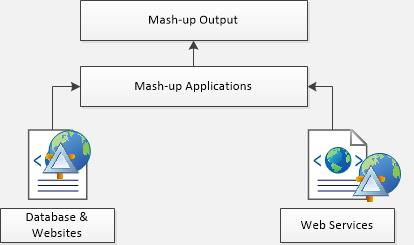
\includegraphics[scale=1.2]{chapter2/mashup_arch}
\caption{Data Mashup Architecture }
\end{figure}

There are many definitions used for mashup technologies, but in all definitions there are two consistent themes which are listed below \cite{fung2012service}.

\begin{itemize}
\item Mashups are very simple to create and easy to deploy. In fact, that business users should be able to create without any great assistance from the IT application developers.
\item Mashups are composed of a selection of easy to integrate data sources. These data sources could consist of either pure data formats such as XML, JSON or CSV, or a combined data and presentation formal (HTML).
\end{itemize}

Through these two themes user can see the basis of a disruptive technology. In this technology the need for agility and self service for the business users intersects with the existing technologies for easily exposing the desired data in an easy and understandable fashion. The mashup technologies span a wide variety of users - such as the consumer using a portal or rich internet app that collects, aggregates and transforms diverse data sets into something new. Mashup technologies also bring in data sources to expose the data and make it easily consumable. Here are the two points; first some of the methods that data is exposed from a structural and protocol perspective, and second some of the different aggregates and portals that are available on the consumer market \cite{arafati2014d}.

\subsubsection{Mashup Data Sources}

A mashup data source can be almost anything one can imagine including an in-house database, a web page or a web service. The main goal of a mashup is to easily consume data, to the point that a business user can create a mashup \cite{gomadam2012data}. This means that most data sources that are commonly used in mashups expose the data by one of the following mechanisms as illustrated in Figure 2.3.

\begin{figure}[H]
\centering
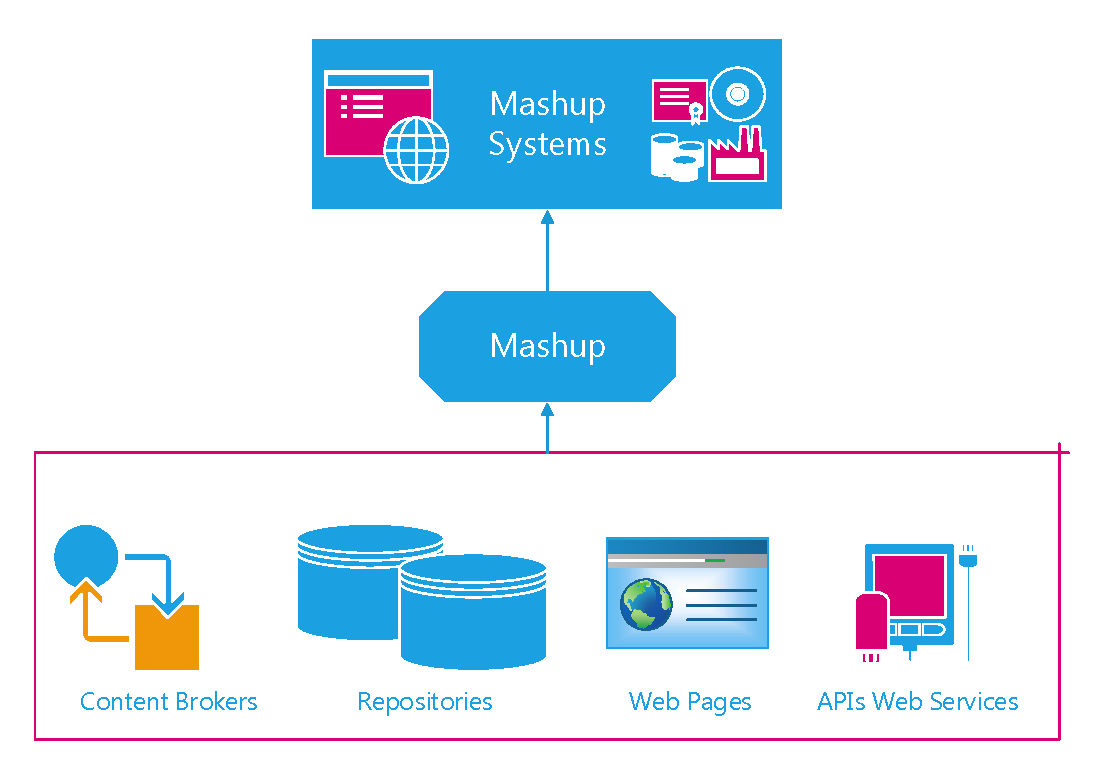
\includegraphics[scale=0.8]{chapter2/mashup}
\caption{Mashup Data Sources }
\end{figure}


\begin{itemize}
\item Rich Site Summary (RSS) or Atom Syndication Format (Atom)
\subsubitem Request is HTTP GET/POST
\subsubitem Response is XML in RSS or Atom Syndication Format.
\item HTML
\subitem Request is HTTP GET/POST
\subitem Response is HTML
\item RESTful web services
\subitem Request is typically HTTP GET/POST
\subitem Response is typically XML or JSON
\item Simple Object Access Protocol (SOAP) web services
\subitem Request is HTTP POST, XML encoded as per the description language
\subitem Response is XML encoded as per the description language.
\end{itemize}

\subsubsection{Enterprise Mashup}

Enterprise based mashups combine business-related heterogeneous data and applications from a myriad of sources (typically a mix of internal data and applications with the externally sourced data, SaaS and web content) to create a full and integrated experience \cite{hoyer2008market}. The general popularity of mashups for both business and consumers has increased in the recent years, particularly with the advent of Web 2.0 and the mass adoption of mobile technologies. Though the early mashups were heavily consumer based, it was quickly and easily determined how to create enterprise mashups to ease the consolidation of functionality onto one page that is usually found across many. This  offers serious benefits and real business opportunities for companies of all shapes and sizes anywhere in the world \cite{he2014enhancing}.

Enterprise mashups can typically be divided into 3 segments:
\begin{itemize}
\item  A presentation layer mashup presents content from various remote sources together in one unified view.
\item  A data mashup which combines, manipulates and ties together disparate data sources and presents in a single unified view. 
\item  Process mashup, which enables the users not just to mashup data sources, but also business processes, allowing customisation of process design and invoking business logic across multiple applications. 
\end{itemize}

As the techniques for creating such mashups have grown and matured, more and more companies are building business models around mashups. To capture a major share in this quickly evolving market, enterprises, software vendors and solution providers need to move quickly, and develop the mashup strategy which incorporates an entire ecosystem of data and mashup technology.


\subsubsection{Client Side Mashup}

Mashups are inherently designed in two different architectures, depending on where the processing and data integration takes place in the system. If this is the case then once the final result has been produced on the server, it is pushed to the client side for visualisation. Alternatively, both the integration and visualisation tasks can take place in the clients browser - resulting in a client-side mashup instead \cite{yu2008understanding}. The client side architecture has significant disadvantages (less security, less reliability and poorer performance to name a few) it still provides a faster user experience- with significantly less load on the servers side and much easier development. To do this, multithreading is required. This is the technique has been used by desktop and server based applications alike to help increase performance levels while performing on concurrent long running tasks \cite{patel2015novel}. 

The developers can now take advantage of multithreading JavaScript support within browsers (HTML5 introduced this feature as the Web Worker API). In later instalments, will go into more detail on this feature, and how it can be used in efficient client side mashup development focusing on process integration (PI), data integration (DI) and data representation (DR). The mashup usually refers to music or vocal editing and it is a single composition created from different songs, however data or web mashups, in a similar spirit, originated from the re-use of existing data sources or web applications, the emphasis being on graphical user interfaces and programming-less specifications. As described in \cite{eick1999visualizing}, the concept of mashups originated from the understanding that the number of applications available on the Web and the needs to combine to meet user requirements. A mashup application can be characterised as a lightweight and tactical presentation layer that uses the web platform – Web-Oriented Architecture (WOA)  - in order to integrate multi-sourced applications mashup offering. Figure 2.4 highlights basic mashup application architecture. The mashup data could be retrieved from several sources, i.e. from local databases or data sets or from external repositories, from a website, via crawling, or via a service oriented approach (SOA) through APIs and from other intermediate content brokers \cite{naik2015framework}. 

\begin{figure}[H]
\centering
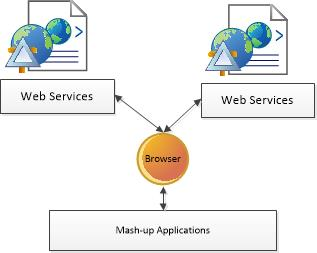
\includegraphics{chapter2/browser_mashup}
\caption{Browser Based Mashup }
\end{figure}

\subsubsection{Server Based Mashup}

The server based mashup application is widely used mashup architecture as there are more benefits and advantages. A server based mashup process, formats and compiles data at a remote site while only transmitting the output of the mashup application. Data can be re-used and high security levels are one of the key advantages of such architecture while requires trust and proxy mashup service resources for computation. Figure 2.5  demonstrate server based mashup application \cite{chen2014development}.


\begin{figure}[H]
\centering
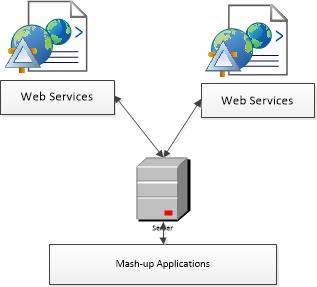
\includegraphics{chapter2/server_baed_mashup}
\caption{Server Based Mashup}
\end{figure}

\subsubsection{Various Mashup Types}

The mashup applications could be categorised into several types; these classifications vary from usage to application development - in all these mashup applications one thing in particular is very important, that is data, and, of course, data is the heart-beat of any mashup application \cite{zhao2011mashup}. The data mashup applications combine similar types of media and information sources into a single representation, or output. All the mashup applications which focus on similar types of data are categorised in this type, a good example could be a news mashup application as the application collects news, stories from different news websites such as, BBC, NY Times and present collected information in one package \cite{li2013customized}. The consumer mashup applications combine different data types, also combines data from different data sources and present application in an integrated view, there are several types of application developed to serve consumers and most commonly cited is housingmaps.com which combines Google maps data with Craigslist housing data in one integrated view \cite{zhao2011mashup}. 

The enterprise mashup applications are slightly different from data mashup, and consumer mashups, as enterprise mashups mostly combine own resources, applications and data with external web services which establishes a collaborative approach among business and developers \cite{liu2011composing}. The above are widely used mashup types however, this list is dynamic and more categories are introduced with time. Client mashups are widely regarded as solving personal situational problems while enterprise mashups focus on collaborative and coordinated problems, consumer and business mashups are used as analogous terms for client mashups and enterprise mashups respectively. The classifications of various mashup systems are highlighted in Table 2.1 \cite{11}.

\begin{table}[h!]
\centering
 \begin{tabular}{||c | c ||} 
 \hline
 \textbf{Client Mashups} & \textbf{Enterprise Mashups}  \\ [0.5ex] 
 \hline\hline
Consumer  & 	Business mashups\\
Front-end  &	Back-end mashups\\
Web Page Customisation &	Process \\
Horizontal  & 	Vertical \\ [1ex] 
 \hline
 \end{tabular}
 \caption{Classification of Mashup Systems}

\end{table}

Web page customisation mashups are more interface oriented mashup systems which helps the presentation layout of web application development; a good example is the BBC website where user can drag content boxes to see stories that are important. Process mashup helps in computation elements of application for example, data aggregations and sequential process automation \cite{de2009process}. Front-end mashup application helps in improving front-end by adding/deleting website widgets and gadgets; a good example of this type is iGoogle and Netvibes. Back-end mashup applications combines web accessible data and services into more useful web services that can be accessed easily for further re-use such as Kapow and Yahoo Pipes \cite{pipes}. Horizontal mashup applications are dependent on execution of a previous service within the application in order to represent the information, for example on a travel website, the web application needs to execute and list all destinations and then to be displayed on a map as a kind of horizontal mashup application \cite{zhao2012design}. Vertical applications depended on application output rather than execution as the next part of the application then process further information as instructions received, and the application does not provide information by itself \cite{zhao2012design}. Various types and architecture of these mashup and its benefits are discussed and explained above; combination of client side and server side mashup technologies will be utilised in our model development phase.

\section{Web 2.0}

Web 2.0 was first introduced during a conference between O'Reilly and Media Live \cite{o2009web}, and joins a new generation of web application, and represents both a practice and a technology benchmark. It has improved on its predecessor Web 1.0 in a multitude of ways, and has become more interactive and dynamic than ever before. This new improved application allows users to both access content from a website, and contribute to it - allowing to keep up with the site's latest content even if it doesn't have the latest web page version. It has also been improved for developers, allowing users to create new web applications that draw on data, information or services that are available on the internet. A more comprehensive list of differences between Web 1.0 and Web 2.0 technologies are undertaken by Cormode et al \cite{cormode2008key}. 

This new technology is focused on the reuse and open standard based technologies with both scalability and flexibility in new dynamic environments. Web 2.0 technologies can not only help with the creation of standard web application, but it can also aid in the construction of circumstantial applications, which can explore enterprise applications and data for business users and customers. It can help limit the possibility of information  overload while adding a new dimension of modernisations for businesses and end users. It has improved on various other aspects of Web 1.0, including commercial impact, the re-usability of applications and data, and even user friendliness. These new technologies are developed and positioned on uncomplicated programming imitations, and these can help rapidly accelerate its time to market, and improve the usability of enterprise assets \cite{21}. From the conference, O'Reilly Media have given seven principles, and fulfilling these will qualify a company or application to be categorised as a Web 2.0 application. The success of the Web 2.0 application will be judged on these principles \cite{webtim}: 

\begin{itemize}
\item Services, not packages software with cost-effective scalability
\item Control over unique, hard to recreate data sources that get richer as more people use
\item Trusting users as co-developers
\item Harnessing collective intelligence
\item  Leveraging the long tail through customer self-service
\item Software above the level of a single device
\item Lightweight user interfaces, development and business models.  
\end{itemize}


The core of the Web 2.0 application is to encourage an individual's freedom, not only to create, but to annotate, comment upon, index and share the content within it - completely bypassing the more traditional models of editorial control, centralised publishing and professional indexing. The flow of content is now no longer a strictly top down operation, now flowing from classic producers to consumers. The traditional distinction between the content producers and the consumers is blurred, and a new bottom up movement ban be instigated, one which facilitates self-organisation. Once ordinary users get more involved in the process of content creation, self-organising communities emerge. To support this, only need to look at Wikipedia - which builds on the tight involvement of users, sense of community and deep dedication to developing a large and unprecedented knowledge repository. The same responses to other community driven websites, such as blogs, wikis and podcasts, and in all of these the sum of community knowledge is larger than that of the individuals. This harnessing of collective intelligence is an essential part of the Web 2.0 application, with the intention of turning the internet into a form of global brain. While anyone on the internet can edit the existing pages of wikis and add new pages at any time, more scientific articles found in Wikipedia are fully comparable with the corresponding information from sources such as the Encyclopedia Britannica in terms of accuracy \cite{berthon2012marketing}.

\subsection{Web 2.0 Models}

The beauty of Web 2.0 applications are embedded in real business models \cite{webtim}. For example, the fact that Google has recently expanded dramatically and the credit largely goes to the search and advertisement market, which has the highest growth potential on the internet \cite{21}. Because of its success and versatility, a great number of studies have contributed to many Internet business models. It is because of this that Afuah and Tucci \cite{22} defined two classifications of business models. The first classification is adopted from \cite{23} and was based on the differences between traditional and Internet business. This included elements such as e-shopping, e-procurement, e-auction, e-mail and information brokering. 

The second classification was initially constructed by \cite{24}, and this mainly presented the taxonomy of the various categories of business models, including brokerage, advertising, informatory, merchant, manufacturer, affiliate, community, subscription and utility. But this itself has caused issues, as there is rarely a categorisation of Web 2.0 business applications based on the value, it can generate for both the customers and the service providers. Based on both user involvement, service provider efforts and the various sources of revenue, the following factors to act as differentiators between the different types of Web 2.0 business models. This measures the degree of consumer participation in the design, development, storage and reuse of the systems and application on the Web 2.0 horizon. The learning management system (or LM for short) is designed to raise learning management activities while promoting the acquiring of data, transfer of data and sharing of the content and information. Internet based businesses may already support users with some forms of learning management participation, such as free exertion of knowledge management and the regulated processes of authenticating the correctness of data. This syndrome the rationalised processing of the knowledge network and learning commerce, and even knowledge capture technology such as relationship recognition between new and previous content \cite{sclater2008web}.

As an example, Wikipedia is a huge encyclopedia which was collectively created by many of its users from across the world, and offers a recognised process for users to add and edit knowledge on the Internet. Any user signed up can log in, edit and offer corrections on any published article, and because of this the content of Wikipedia is being constantly monitored and improved. It is logged at making thousands of changes an hour, all of which are recorded in article histories. Any inappropriate uploads or changes are quickly moderated and removed, and repeat offenders can be blocked from changing articles in the future. Users can also add hyperlinks for readers reference, and all articles are arranged in proper categories for ease of reference. All articles that are arranged this way benefit from the search function to allow readers to find information easily \cite{aghaei2012evolution}. Businesses often price applications or commodity depending on cumulative sum of the cost of assets, crude elements and labour for generating the objects. A Web 2.0 user will consume large sums of resources in the applications, internet bandwidth, research and development and knowledge generation \cite{shang2011understanding}.

\subsection{Web 2.0 Usage}

With the creation of Wikipedia, the internet fast became home to a revolutionary website; a free, online encyclopedia backed by an expert team comprised of writers editors and proofreaders. But in the early days the results received were poor at best, and the team had to devise a new concept in which readers are allowed to self-select what roles they wished to play, what content to create and what the content was. This change resulted in a group of people who were extremely enthusiastic about the project and had a vested interest in the quality of the output, and this brought the quality of the online encyclopedia to the surface and revealed its true potential. This success triggered a phenomenal outbreak of social encyclopedias, Facebook, Flickr and Youtube, and this industry is still growing. At the heart of these new web-based solutions to find a web of social network services, spawned with the idea of building more of these online communities with people who share interests and activities, or wish to explore the interests and activities of others \cite{kamel2007emerging}. Web 2.0 is yet another new revolution in the direction of the computer industry and solutions for businesses. This was caused by the movement of company intelligence and the management of business ideas, with the internet as its new platform. In an attempt to understand the rules for success on this new platform, a set of experiments were applied to a heterogeneous mixture of relatively familiar emerging technologies, all based around the idea of harnessing the collective intelligence of crowds to give information new value \cite{webtim}. 

This new idea about the creation and collaboration of the collective intelligence when placed into a database sitting behind the internet technologies is crucial for the success of the complex group of different solutions known as Web 2.0. It is safe to say that Web 2.0 is a completely open concept, which does not have any hard boundaries, but instead has a gravitational core. A simple set of principles and practices tie together within the internet as a platform for the solutions. The term Web 2.0 refers to the cumulative changes in the ways multiple software developers and end-users alike use the internet. It refers to an attempt to conceptualise the exact significance of a set of outcomes that are enabled by these internet technologies \cite{boateng2014web}. The industry standard technology used for Web 2.0 is Asynchronous JavaScript and XML (AJAX). This is a method that allows a minimal data exchange with the back room servers, and allows a group of interconnected web development techniques to be used on the client side to create interactive and responsive web applications or rich internet applications. Because this system has a dynamic and immediate update of the pages content in the background, without interfering with the displays of the existing live page \cite{webtim}. Whilst a good tool can facilitate work and help in the ease of doing a job, it does not provide new solutions to problems or innovative ways to work. Web 2.0 facilitate users with content creation and service availability - with the advantage of a collective intelligence strongly based on mutual trust but driven by common goals and motivations. Maintaining the content of the internet in this new way breaks away from the traditional page metaphor, and instead relies on the composition of microcontents. Using this technology user can define a whole new set of content building blocks, where blogs are about posts and not pages, and wikis are transformed into endless streams of conversations, revision, amendments and truncation. Podcasts will be shuttled between websites, while RSS feeds diversify players. Once created, these AJAX technology based content blocks can be saved, summarised, addressed, copied, quoted and even built into new projects. This creates a whole new content metaphor, and one that is rising on this original microcontent drive. This allows users to develop the contents completely collaboratively and open it to the world, and it is this openness that is essential to the whole concept \cite{mesbah2012crawling}. 

Web 2.0 concepts are microcontent and openness, but these two elements are only part of a larger strand of concept. Web 2.0 brings out a whole new role for users, putting more of a foundational role on the old wisdom of the crowds argument. This new platform responds to its users in a completely new form of metadata affectionately known as folksonomy - organised on the sets of words generated by the users and attached to the contents of the web \cite{chen2014retracted}. There are a few problems with the idea of wisdom of the crowds, and one of the most prominent of these is the value of the data produced by multiple sources that are so out of any form of control. Web 2.0 gives every user the opportunity to take part in the creation of the massive log of contents in the back end database. The content created is unstructured with dubious accuracy, and this leads to huge and well known problems in the field of knowledge management. However there are a few different approaches to solve these problems. For example in blogs, user can see that the microcontent is signed, albeit usually under a pseudonym, but the author who uses this sign takes full responsibility for the microcontent. The same theory applies to pictures uploaded to Flickr. More of a problem is presented with networks such as YouTube, where on average 100 hours of video is uploaded every minute and it is not possible to organise and review the content \cite{youtube}. This instead puts the entire responsibility with the authors, as is also the case on social networking platforms like Facebook, MySpace and Twitter. In handling content on these platforms, a whole new set of tools and techniques introduced for the creation of wikis, blogs, tagging and feeds, which automatically helps other participants in a network to share links and ideas \cite{auer2007dbpedia}.

\subsection{Enterprise 2.0 - An Overview}

Enterprise 2.0 was a concept first introduced by McAfee in order to showcase how Web 2.0 technologies can be used within enterprises. The focus was to explain how Web 2.0 could make practices and the efforts of knowledge workers more visible. This is in reaction to the initial response to Web 2.0 by the businesses - when introduced it fascinated almost everyone, but it did not seem to register with enterprises. In order to take these (or any) emerging technologies seriously, companies needed to see real case studies of the use of Web 2.0. Case studies in which the application had been studied and analysed from multiple perspectives, including security, consistency or scalability. Enterprise 2.0 need a set of best practice descriptions for its use, and specific guidelines on Web 2.0 technologies within organisation \cite{mcafee2006enterprise}. How was the new technology of Enterprise 2.0 studied and discussed in other areas? While there have not been many in depth qualitative analysis on Enterprise 2.0 within the work context and its impact, there have been multiple studies on the direction, detail, quality and format of social networking systems (particularly Facebook and Twitter). There are even qualitative studies focused on application and real use within business. However in recent years, some managerial journals have published new results of the applied Enterprise 2.0 technology, and some books have even been published with a specific emphasis on providing explanatory guidelines for management in enterprise. While these sources were a considerable jump forward, it does not exhaustively and qualitatively describe how and in which areas this new technology is more efficient for enterprises - or the additional value it can have to cooperative work. This is something that the research literature still lacks - an in depth analysis and explanation of cooperation processes in very complex development environments. This is the sort of thing that needs investigating, by basing the analysis on central concepts such as awareness, trust, openness, sharing through data mashup tools and information visualisation \cite{mcafee2013enterprise}.

However, introducing changes into any organisation is a difficult subject as resistance to change is often immediate and dramatic, without any deeper thought. Organisational culture also impacts the attitudes towards Enterprise 2.0 adoption, because the organisations general attitudes towards collaboration, open communication and information sharing hugely affect the acceptance of Enterprise 2.0 by employees and managers. The common fear the organisations have is that it will lose governance over information, and Web 2.0 tools as perceived as a potential risk, particularly in the field of data loss. This is viewed as a direct result of employees sharing information on blogs or social networking sites. There is also a huge concern for decreased employee productivity, or the possibility that the wrong information will be posted on a network by an employee, or even that employees will write questionable or offensive materials on a network. These fears are what fuels the standardisation of office policies and processes when it comes to social networking and collaborative work - usually opposed. This is particularly true for organisations who operate under a command and control culture \cite{williams2013enterprise}. Despite all of these barriers, some organisations are not only starting to use Web 2.0 technology, but are also leveraging it to change management practice and organisational structures. Those organisations that have recognised the innovations that Web 2.0 technology represented by innovation instead of price have tapped into a priceless idea - using the knowledge (and tacit knowledge) of workforce and therefore encouraging collaboration among knowledge workers using the Enterprise 2.0 tools. Many more organisations are starting to see Enterprise 2.0 technologies as an opportunity to increase company's revenue and margins, and see its many benefits. The undeniable fact is that Enterprise 2.0 is an unavoidable technology - one which is becoming increasingly popular among enterprise specific users, and more so among knowledge workers and digital natives who have grown up with the web \cite{kim2013building}. 

In these modern times the nature of work is constantly evolving, and being driven by the Web 2.0 technologies that enable and enhance social activities it has quickly taken on a significant role in the workplace. Enterprise 2.0 has not only become a competitive necessity, now organisations must be ready to use the technology that supports it. After all, simply adopting the technology in a process does not necessarily improve the process by itself. The technology must be fully assimilated into the organisation in order to gain the full competitive advantage and considerations about technological capabilities, willingness of adoption and organisational size must all be taken into consideration, helping in the evaluation of the organisations readiness for Enterprise 2.0 \cite{mcafee2009enterprise}.

\section{Data Storage}

Data warehouses can be characterised in a number of different ways, but for now with a very basic principle. A data warehouse is made up of a complex architecture including data sources, data staging areas, operational data stores, some global data warehouses and even client data marts and this makes an incredibly complex thing to modify \cite{berg2004qualitative}. A new business process is often the catalyst for change within the data warehouse and these changes trigger the need for new software. The warehouse is then used to define the requirements for those software systems so it can be designed to co-exist or integrate. There have been many hundreds of hours spent researching and working on the industry, but addressing the delicate alignment between business processes and information technology has only been mentioned in passing \cite{rabl2012solving}. Instead the majority of software developers are continuing in ignorance of the business processes required or unable to read the models provided (this is not surprising, as different modeling languages all use different diagrams and notations, and are all used in both domains). Instead of letting this continue. The solution here is to fulfil the needs of developers and the business users by applying more business-oriented approaches to the development of a new data analysis solution.

Most of the existing visualisation systems \cite{fry,north2000snap,spotfire,tableau} are focused on the visualisation aspects of the data while limited attention is given to re-use of the visualised content. The beauty of the modern applications are the re-use of the data elements. There is a knowledge gap as how could we utilised and re-use visualised content generated by visualisation tools.

\section{Summary}

Existing techniques and technologies in acquisition and data analysis are discussed in the first part of the chapter. Web and data mining techniques are further discussed with more insights to the mining procedures adapted in the mashup and Web 2.0 scenarios. Existing models, systems and frameworks utilised in information visualisation are highlight from various angles. How existing tools are going to be linked with the proposed model. Key elements of the proposed research such as multi-coordinate visualisation and multi-attribute visualisation techniques are explored. The importance of Web 2.0 demonstrated along with various references to the current proceedings. Web 2.0 facilitation of the proposed model put forward. The mashup technologies are discussed in detail with various types of mashup architectures available for application development. 

Every company that understands business transactions is closer to understanding clients and their needs; which is one step closer to being able to meet and exceed \cite{price2011best}. And after all, happy customers leads to happy businesses \cite{plassmann2007companies}. That's why the next chapter will propose a compound information visualisation model which will help in answering most of the data problems. A comprehensive four step visualisation model is proposed in the next chapter. 
